% ----------------------------------------------------------
\chapter{Estado da Arte}
% ----------------------------------------------------------

\section{Métodos de Escavação}

Há diversas formas de se executar túneis, tanto profundos quanto superficiais. Durante a escolha do método de escavação, o engenheiro deve levar em conta diversos fatores, tais como: geometria da seção, comprimento do túnel, condições geológicas, nível da água, restrições quanto às vibrações, estabilidade da cavidade, riscos de assentamentos superficiais, hipóteses de projeto, segurança dos operários, viabilidade ambiental e econômica. Em vista dessa complexidade é possível utilizar mais de um método de escavação ao longo do eixo do túnel. A \autoref{metodos_escavacao} resume os principais métodos de escavação.

\begin{figure}[H]
	\begin{center}
		\includegraphics[scale = 1]{0301-métodos de escavação de túneis.pdf}
	\end{center}
	\caption{\label{metodos_escavacao} Métodos de escavação de túneis}
\end{figure}

Os métodos se dividem em dois grandes grupos: 1) não mecanizados (convencionais) e 2) mecanizados. A diferença é que este último é caracterizado pela presença de tuneladoras, que são máquinas especializadas em adentrar a frente de escavação. Os métodos ditos “não mecanizados”, não possuem essas máquinas especializadas, e podem ser agrupados em: vala recoberta, escavação simples e desmonte de rocha.

\subsection{Vala recoberta}

O método da vala recoberta é utilizado preferencialmente para túneis superficiais (conhecido também, nas cidades, como método a céu aberto). Pode ser executado de duas formas: direta (\textit{Cut and Cover}) ou invertida (\textit{Cover and Cut}). A \autoref{vala_recoberta} e \autoref{etapa_execucao_vala_recoberta} ilustram esse método.

\begin{figure}[H]
	\begin{center}
		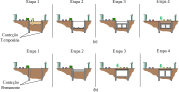
\includegraphics[scale = 0.8]{0302-vala recoberta.pdf}
	\end{center}
	\caption{\label{vala_recoberta} (a) \textit{Cut and Cover} e (b) \textit{Cover and Cut} (adaptado de: \citeonline[p. 5-2]{FederalHighwayAdministration2009})}
\end{figure}

\begin{figure}[H]
	\begin{center}
		\includegraphics[scale = 1]{0303-etapa de execução pelo método de vala recoberta direta.jpg}
	\end{center}
	\caption{\label{etapa_execucao_vala_recoberta} Etapa de execução pelo método de vala recoberta direta no projeto \textit{Nordhavnsvej}, em Compenhague, Dinamarca (fonte: \citeonline[p. 1]{ROADTRAFFIC-TECHNOLOGY2019})}
\end{figure}

Como o presente trabalho está delimitado aos túneis profundos esse método de escavação estará fora do escopo desta tese. Além disso, o comportamento mecânico desse tipo de túnel é diverso dos profundos que, tal como será visto no Capítulo 4, mobilizam a resistência do maciço na estabilidade da cavidade.


\subsection{Escavação simples}


\subsection{Desmonte de rocha}

\subsection{Tuneladora}


\subsection{Cravação de tubos}



\section{Pré-suportes}



\section{Revestimento de túneis}



\section{Principais aspectos considerados em estudos numéricos recentes de túneis}




